\documentclass[a4paper,14pt]{extreport}
\usepackage[left=1.5cm,right=1.5cm,
    top=1.5cm,bottom=2cm,bindingoffset=0cm]{geometry}
\usepackage{scrextend}
\usepackage[T1,T2A]{fontenc}
\usepackage[utf8]{inputenc}
\usepackage[english,russian,ukrainian]{babel}
\usepackage{tabularx}
\usepackage{amssymb}
\linespread{1.5}
\usepackage{color}
\usepackage{amsmath}
\usepackage{mathrsfs}
\usepackage{listings}
\usepackage{graphicx}
\graphicspath{ {./images/} }
\usepackage{lipsum}
\usepackage{xcolor}
\usepackage{hyperref}
\usepackage{tcolorbox}
\usepackage{tikz}
\usepackage[framemethod=TikZ]{mdframed}
\usepackage{wrapfig,boxedminipage,lipsum}
\mdfdefinestyle{MyFrame}{%
linecolor=blue,outerlinewidth=2pt,roundcorner=20pt,innertopmargin=\baselineskip,innerbottommargin=\baselineskip,innerrightmargin=20pt,innerleftmargin=20pt,backgroundcolor=gray!50!white}
 \usepackage{csvsimple}
 \usepackage{supertabular}
\usepackage{pdflscape}
\usepackage{fancyvrb}
%\usepackage{comment}
\definecolor{ggreen}{rgb}{0.4,1,0}
\definecolor{rred}{rgb}{1,0.1,0.1}
\definecolor{aquamarine}{rgb}{0.5, 1.0, 0.83}
\definecolor{amber}{rgb}{1.0, 0.75, 0.0}
\definecolor{babyblue}{rgb}{0.54, 0.81, 0.94}
\usepackage{array,tabularx}
\usepackage{colortbl}

\usepackage{varwidth}
\tcbuselibrary{skins}
\usepackage{fancybox}

\usetikzlibrary{calc}
\makeatletter
\newlength{\mylength}
\xdef\CircleFactor{1.1}
\setlength\mylength{\dimexpr\f@size pt}
\newsavebox{\mybox}
\newcommand*\circled[2][draw=blue]{\savebox\mybox{\vbox{\vphantom{WL1/}#1}}\setlength\mylength{\dimexpr\CircleFactor\dimexpr\ht\mybox+\dp\mybox\relax\relax}\tikzset{mystyle/.style={circle,#1,minimum height={\mylength}}}
\tikz[baseline=(char.base)]
\node[mystyle] (char) {#2};}
\makeatother




\usepackage{float}
\usepackage{wrapfig}
\usepackage{framed}
%for nice Code{
\lstdefinestyle{customc}{
  belowcaptionskip=1\baselineskip,
  breaklines=true,
  frame=L,
  xleftmargin=\parindent,
  language=C,
  showstringspaces=false,
  basicstyle=\small\ttfamily,
  keywordstyle=\bfseries\color{green!40!black},
  commentstyle=\itshape\color{purple!40!black},
  identifierstyle=\color{blue},
  stringstyle=\color{orange},
}
\lstset{escapechar=@,style=customc}
%}


\begin{document}
\pagecolor{white}
\begin{titlepage}
  \begin{center}
    \large
    Національний технічний університет України \\ "Київський політехнічний інститут імені Ігоря Сікорського"


    Факультет Електроніки

    Кафедра мікроелектроніки
    \vfill

    \textsc{ЗВІТ}\\

    {\Large Про виконання лабораторної роботи №1\\
      з дисципліни: «Вакуумна та плазмова електроніка»\\[1cm]

        ДОСЛІДЖЕННЯ ФОТОЕФЕКТУ


    }
  \bigskip
\end{center}
\vfill

\newlength{\ML}
\settowidth{\ML}{«\underline{\hspace{0.4cm}}» \underline{\hspace{2cm}}}
\hfill
\begin{minipage}{1\textwidth}
Виконавець:\\
Студент 3-го курсу \hspace{4cm} $\underset{\text{(підпис)}}{\underline{\hspace{0.2\textwidth}}}$  \hspace{1cm}З.\,Ю.~Рибін\\
\vspace{1cm}

Перевірив: \hspace{5.9cm} $\underset{\text{(підпис)}}{\underline{\hspace{0.2\textwidth}}}$  \hspace{1cm}О.\,М.~Бевза\\

\end{minipage}

\vfill

\begin{center}
2021
\end{center}
\end{titlepage}



\textbf{Мета роботи}: Дослідження вольт-амперних і світлових характеристик фотоелементів для
видимого спектру світла.
\begin{center}\textbf{Завдання}\end{center}\par
\newtcbox{\xmybox}[1][red]{on line, arc=7pt,colback=#1!10!white,colframe=#1!50!black, before upper={\rule[-3pt]{0pt}{10pt}},boxrule=1pt, boxsep=0pt,left=6pt,right=6pt,top=2pt,bottom=2pt}

1 Зняти ВАХ для 4-х значень довжин хвиль вибравши з набору: 200 нм, 400 нм, 440 нм, 470
нм, 520 нм, 580 нм, 610 нм, 650 нм, 700 нм, 750 нм на вибір при інтенсивності 50\% та 100\%. Побудувати окремо два сімейства кривих для 50\% та 100\% інтенсивності для 3-х різних матеріалів мішені (на вибір). Значення для графіків брати з показань у вікнах «Напруга зміщення» та «Струм».\\

2 Зняти світлові характеристики. Побудувати сімейство кривих залежності
Струм(інтенсивність світла) для довжин хвиль 200 нм, 400 нм, 440 нм для мішені з натрія (або іншого матеріалу фотомішені на вибір). Значення для графіків брати з показань у вікнах «Струм» та «Інтенсивність».\\

3 Побудувати сімейство кривих залежності Енергія(частота) при інтенсивності 50\% на
всьому інтервалі частот для матеріалів мішені: натрій, цинк, мідь, платина, кальцій, магній.\\

\newpage
\begin{center}\textbf{Таблиці з даними}\end{center}\par

\begin{figure}[h]
\caption{Таблиця 1. ВАХ для натрію}
\center{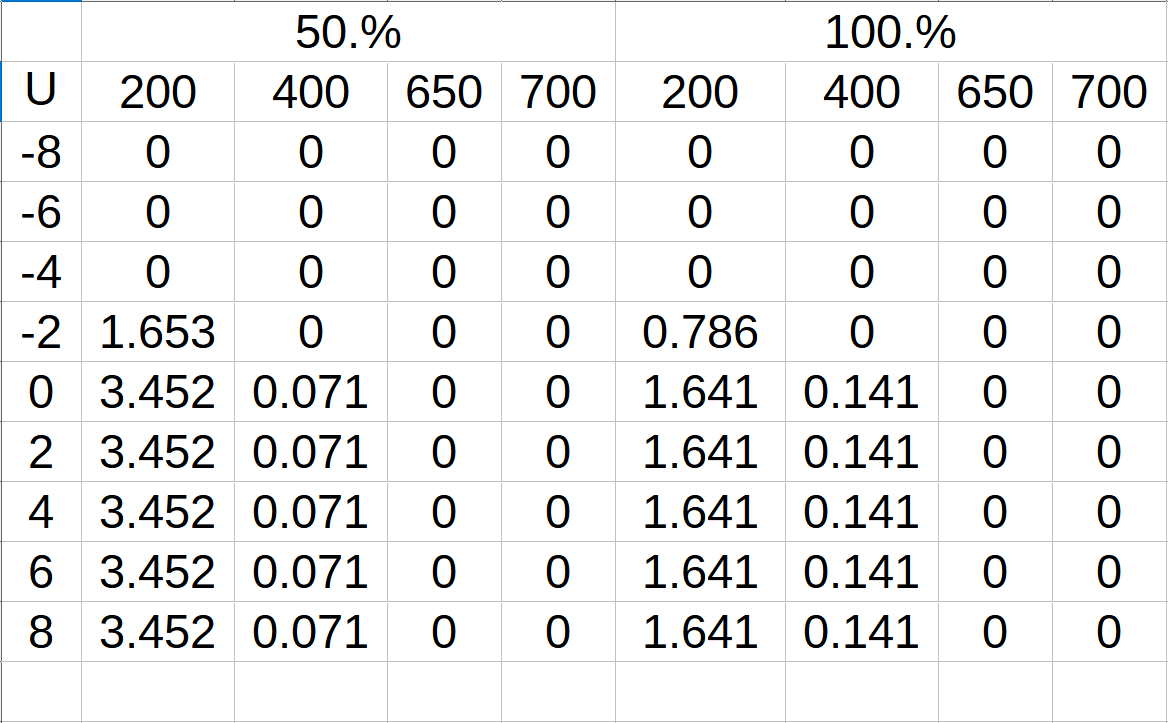
\includegraphics[width=0.6\linewidth]{t_na1.png}}
\end{figure}

\begin{figure}[h]
\caption{Таблиця 2. ВАХ для  цинку}
\center{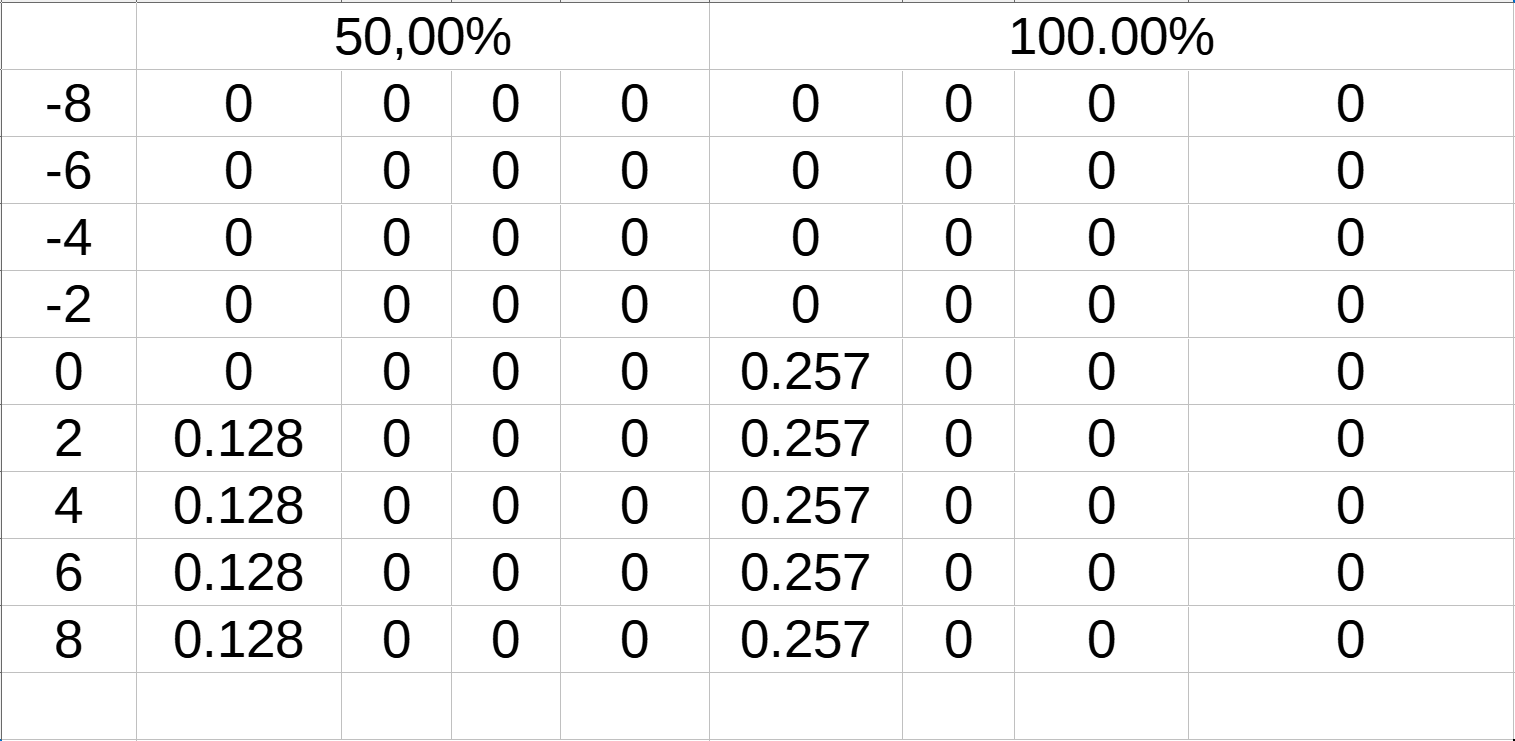
\includegraphics[width=0.6\linewidth]{t_cu1.png}}
\end{figure}

\begin{figure}[h]
\caption{Таблиця 3. ВАХ для міді}
\center{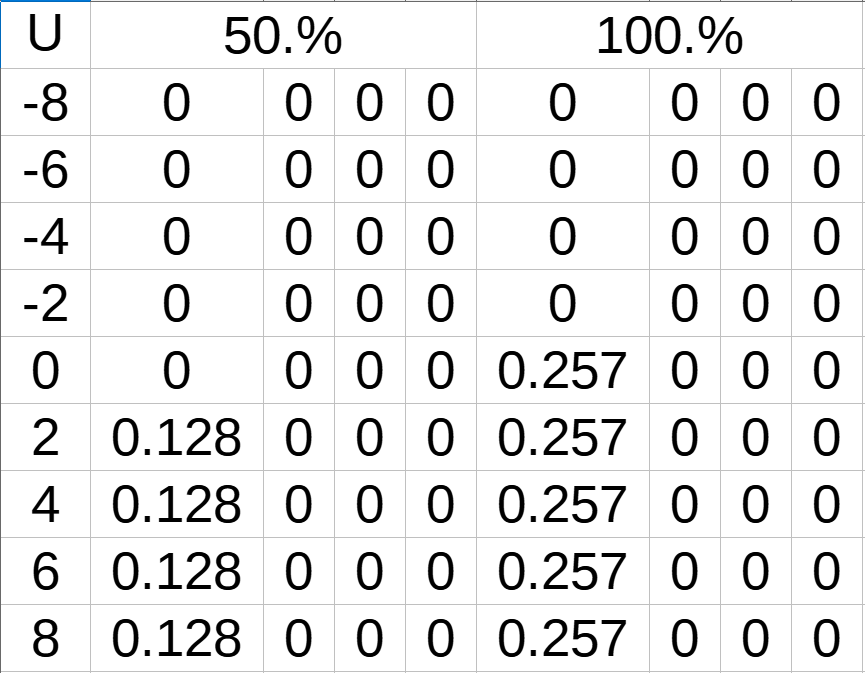
\includegraphics[width=0.5\linewidth]{q.png}}
\end{figure}

\begin{figure}[h]
\caption{Таблиця 4. Світлові характеристики}
\center{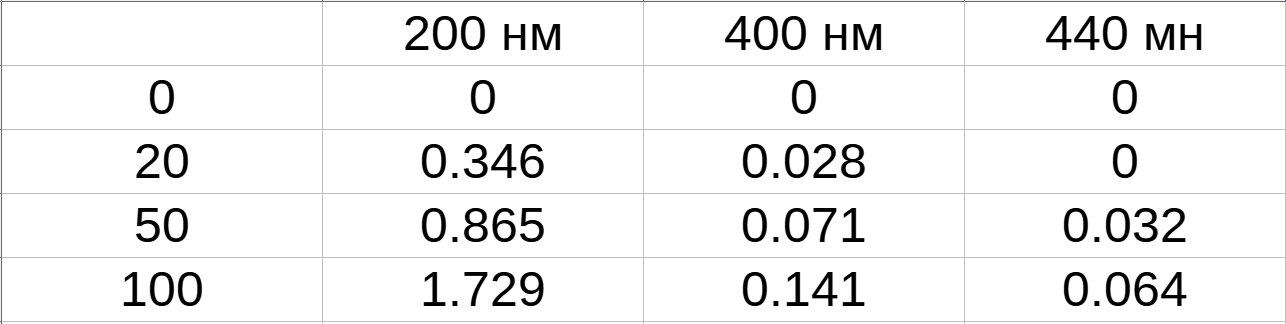
\includegraphics[width=0.6\linewidth]{t_na2.png}}
\end{figure}

\begin{figure}[h]
\caption{Таблиця 5. Залежність енергії електронів від частоти світла}
\center{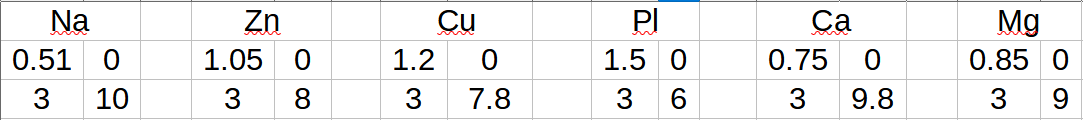
\includegraphics[width=0.6\linewidth]{t3.png}}
\end{figure}





\clearpage
\newpage
\begin{center}\textbf{Виконання}\end{center}\par
Відповідно до п.1, знімаємо ВАХ для значень довжин хвиль 200 нм, 400 нм, 
610 нм та  700 нм для 3-х різних матеріалів мішені.
\begin{center}\fbox{1}\end{center}
\begin{figure}[h]
\center{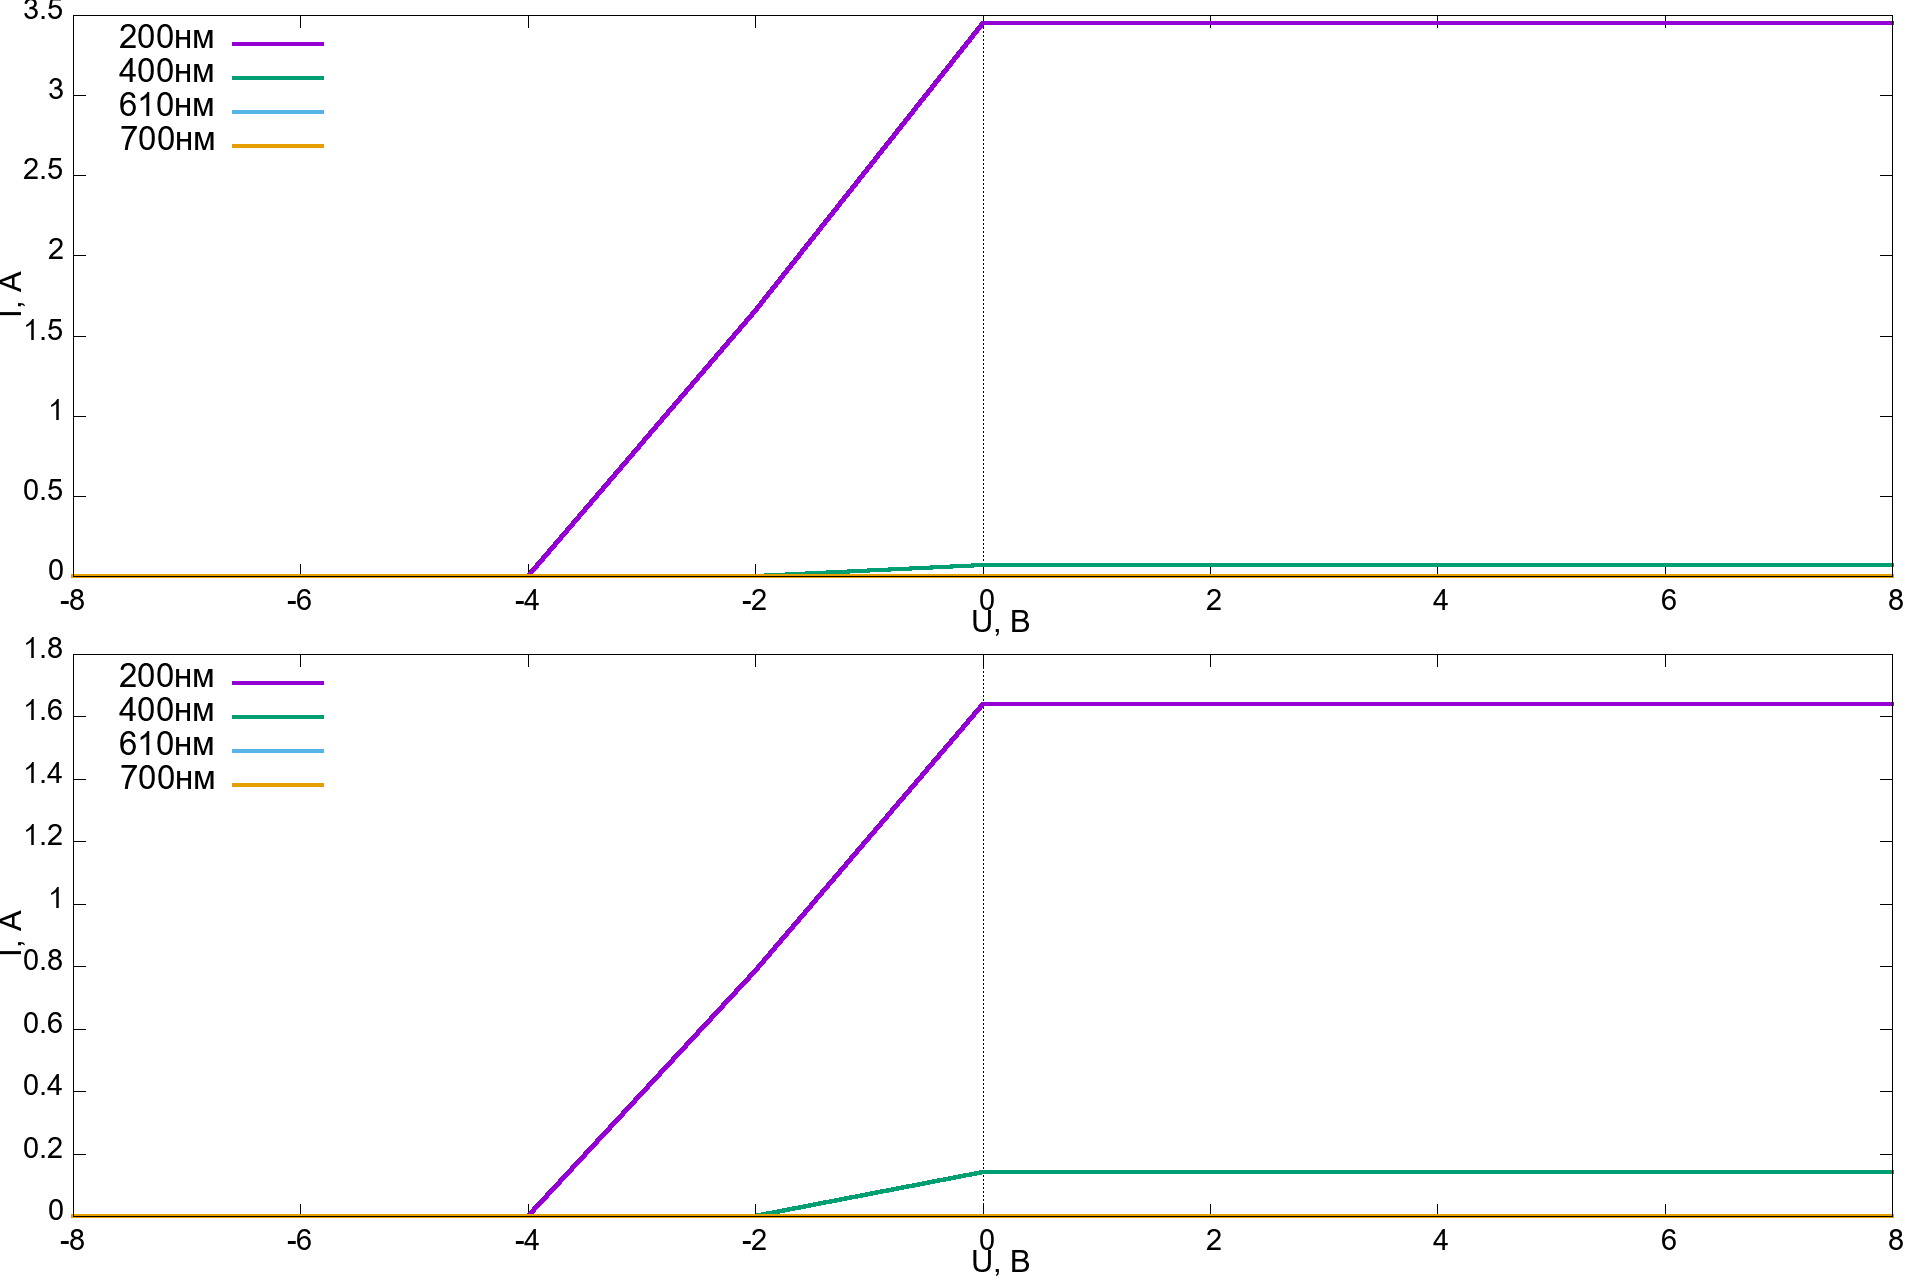
\includegraphics[width=0.8\linewidth]{50-100_Na.png}}
\caption{Сiмейства кривих для 50\% та 100\% iнтенсивностi для Натрію.}
\label{ris1}
\end{figure}

\begin{figure}[h]
\center{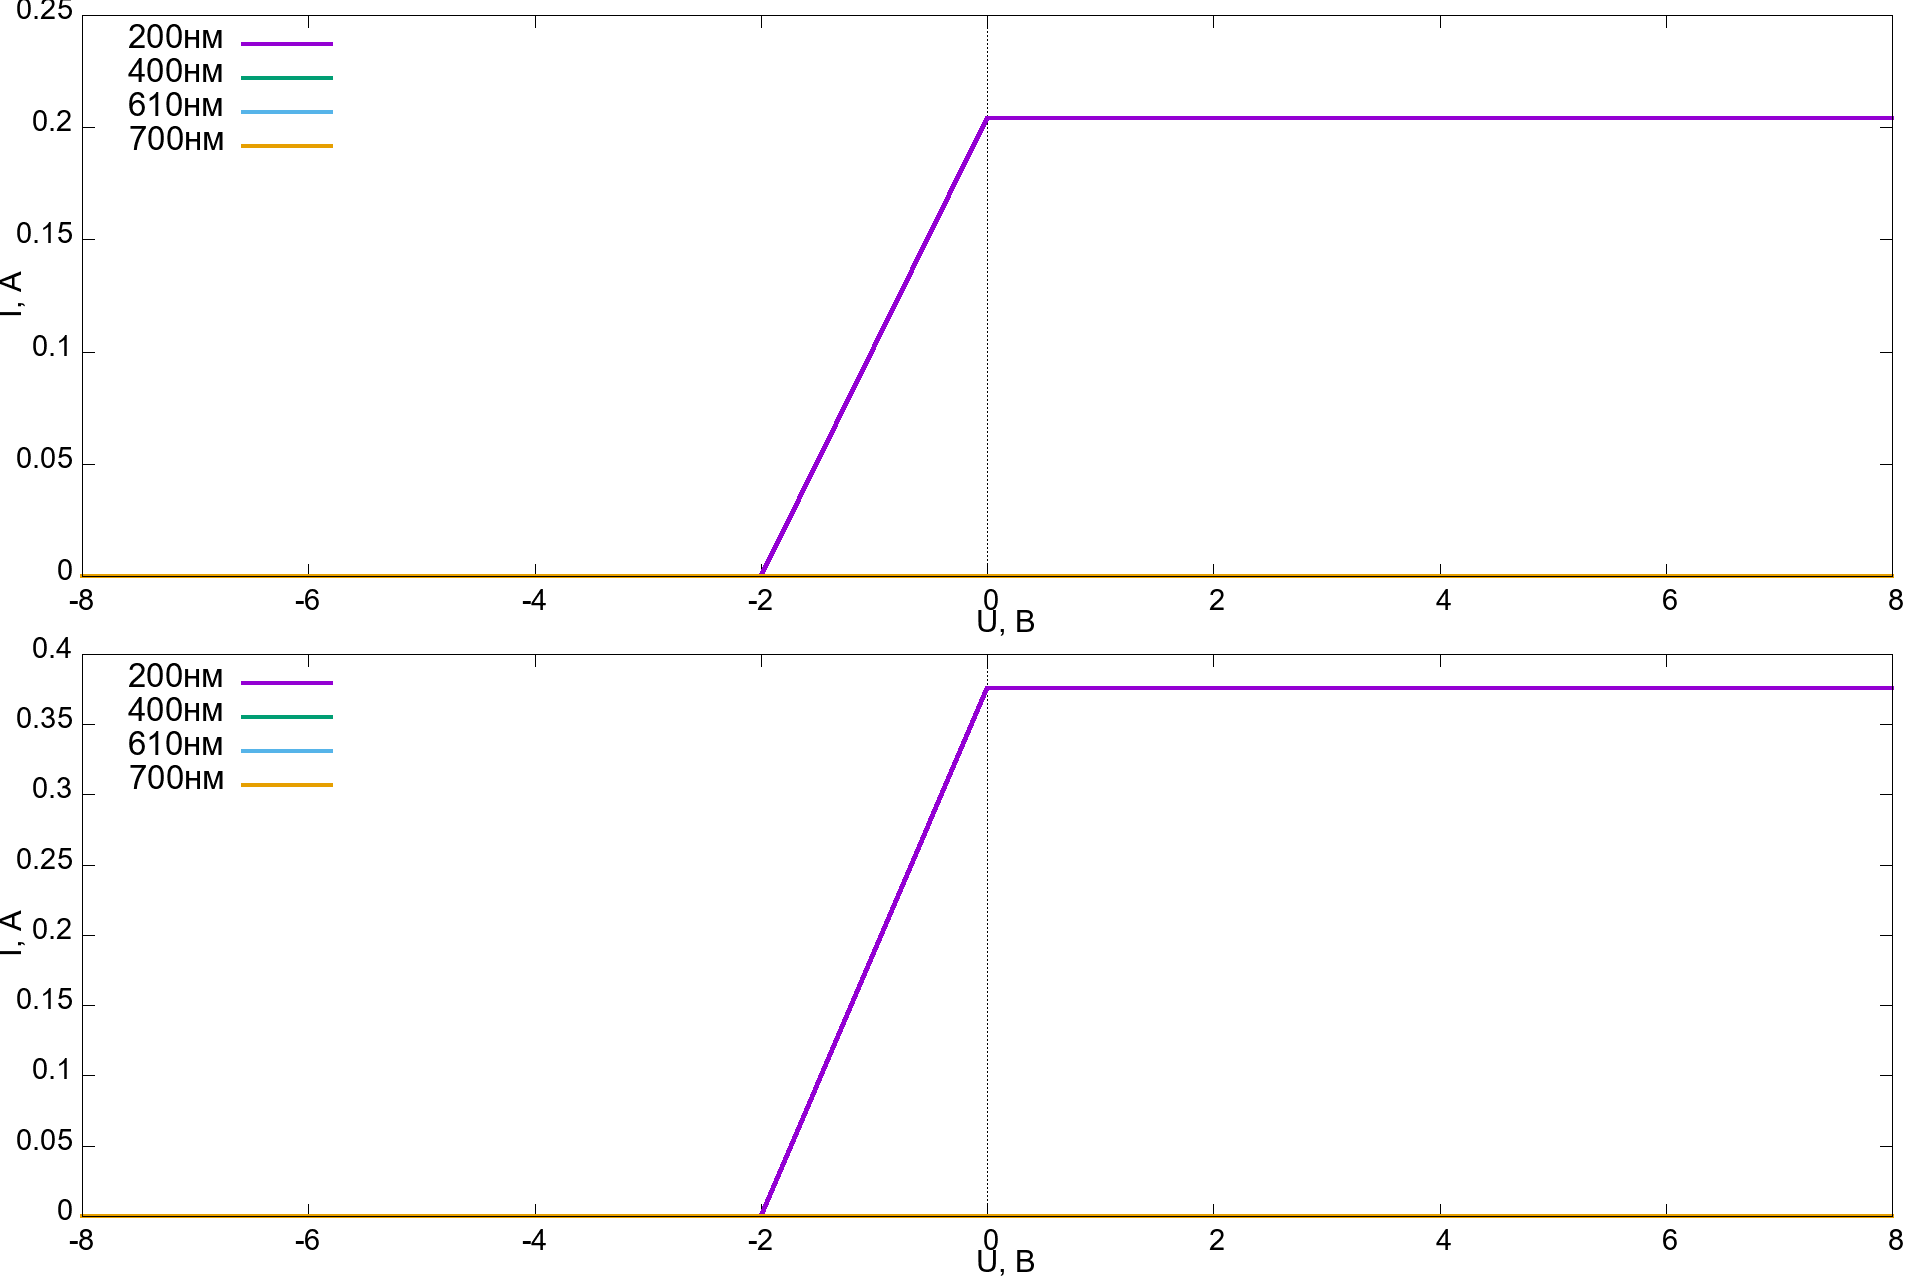
\includegraphics[width=0.8\linewidth]{50-100_Zn.png}}
\caption{Сiмейства кривих для 50\% та 100\% iнтенсивностi для Цинку.}
\label{ris1}
\end{figure}


\begin{figure}[h]
\center{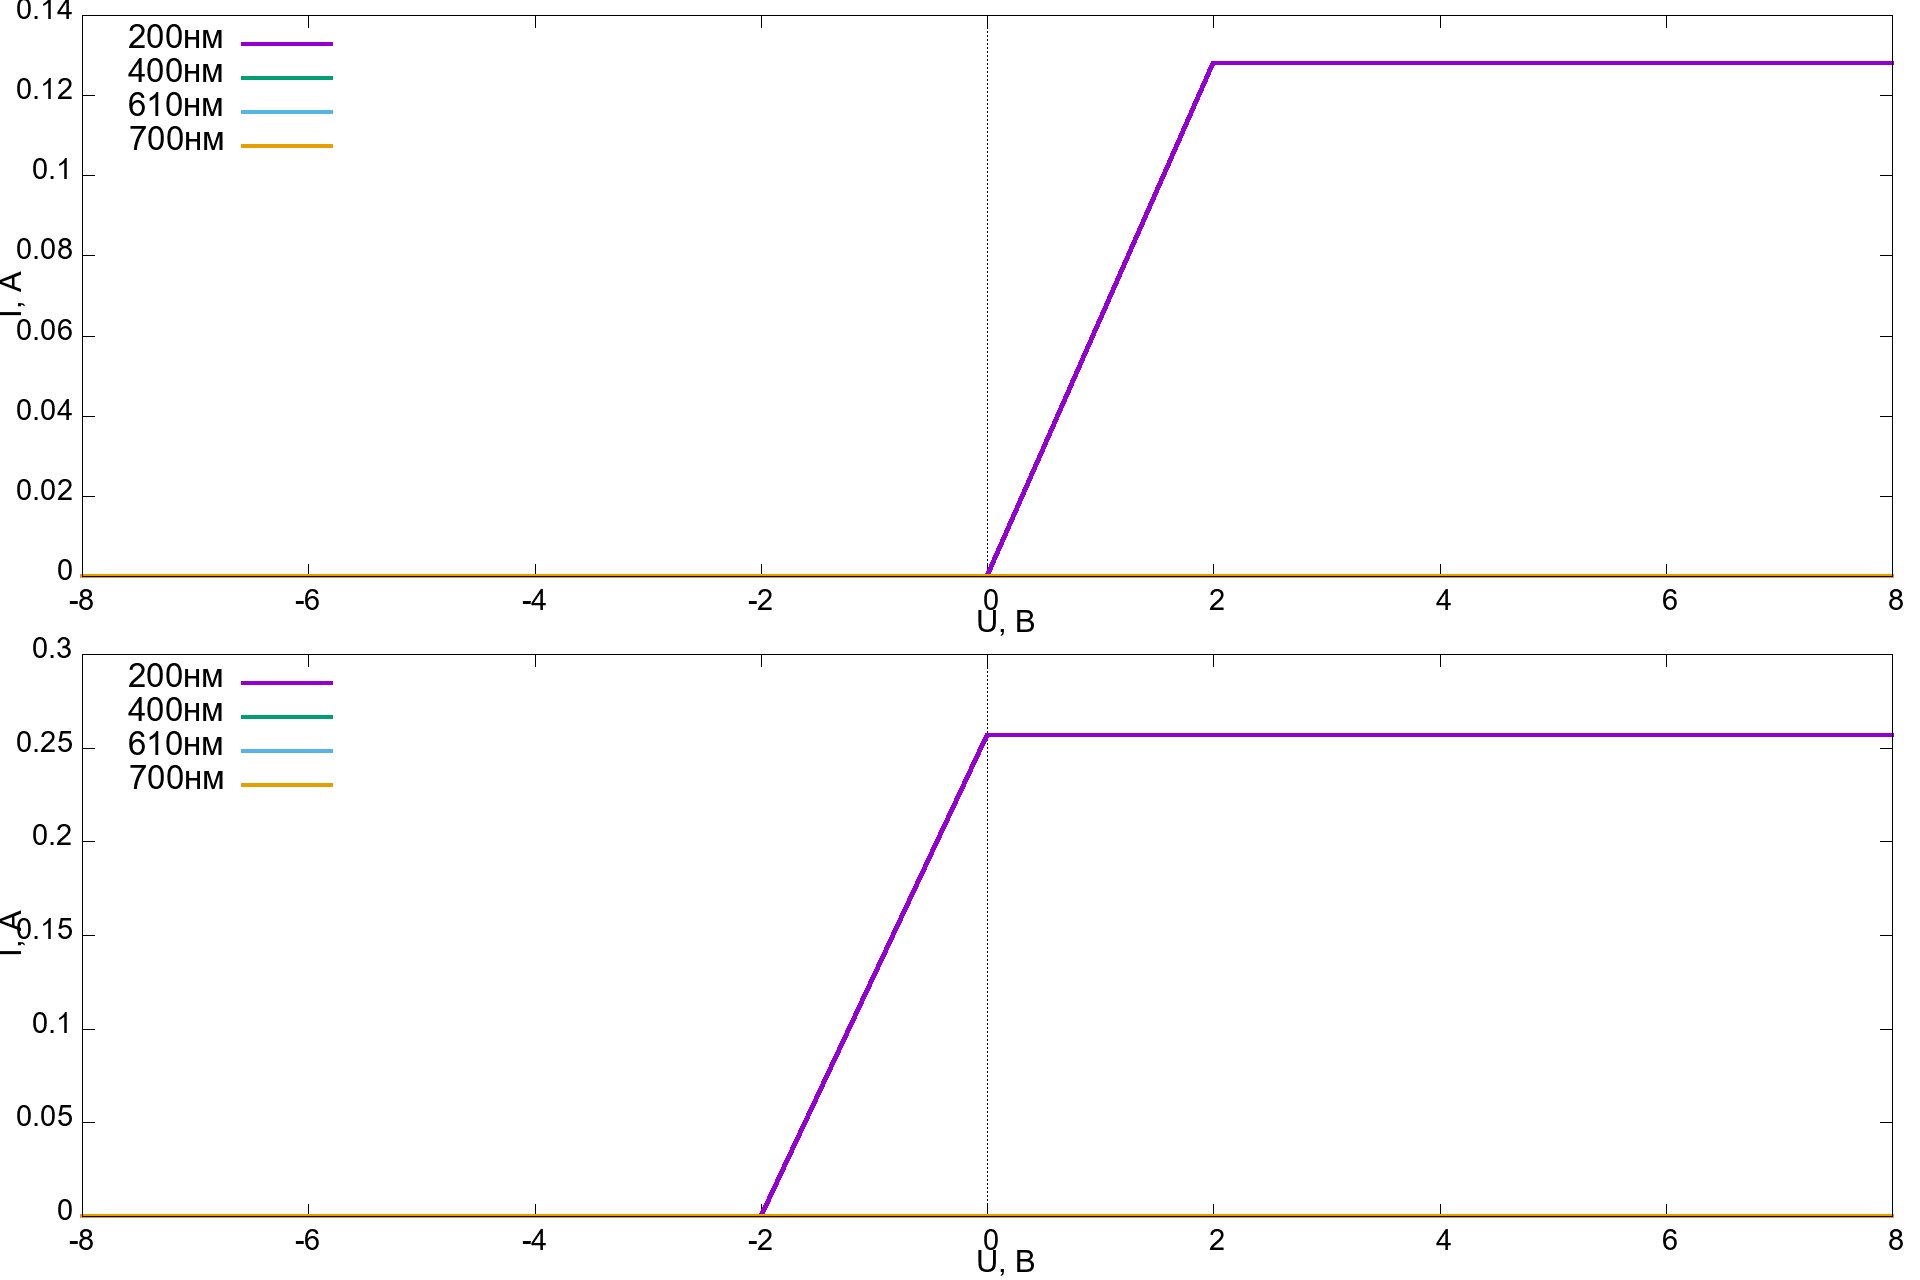
\includegraphics[width=0.8\linewidth]{50-100_Cu.png}}
\caption{Сiмейства кривих для 50\% та 100\% iнтенсивностi для Міді.}
\label{ris1}
\end{figure}





% #######################################
%###                2                ###
%######################################
\clearpage
\newpage
\begin{center}\fbox{2}\end{center}
Далі побудуємо сімейство кривих залежності 
Струм(інтенсивність світла) для довжин хвиль 200 нм 400 нм, 440 нм для мішені з натрія.
\begin{figure}[h]
\center{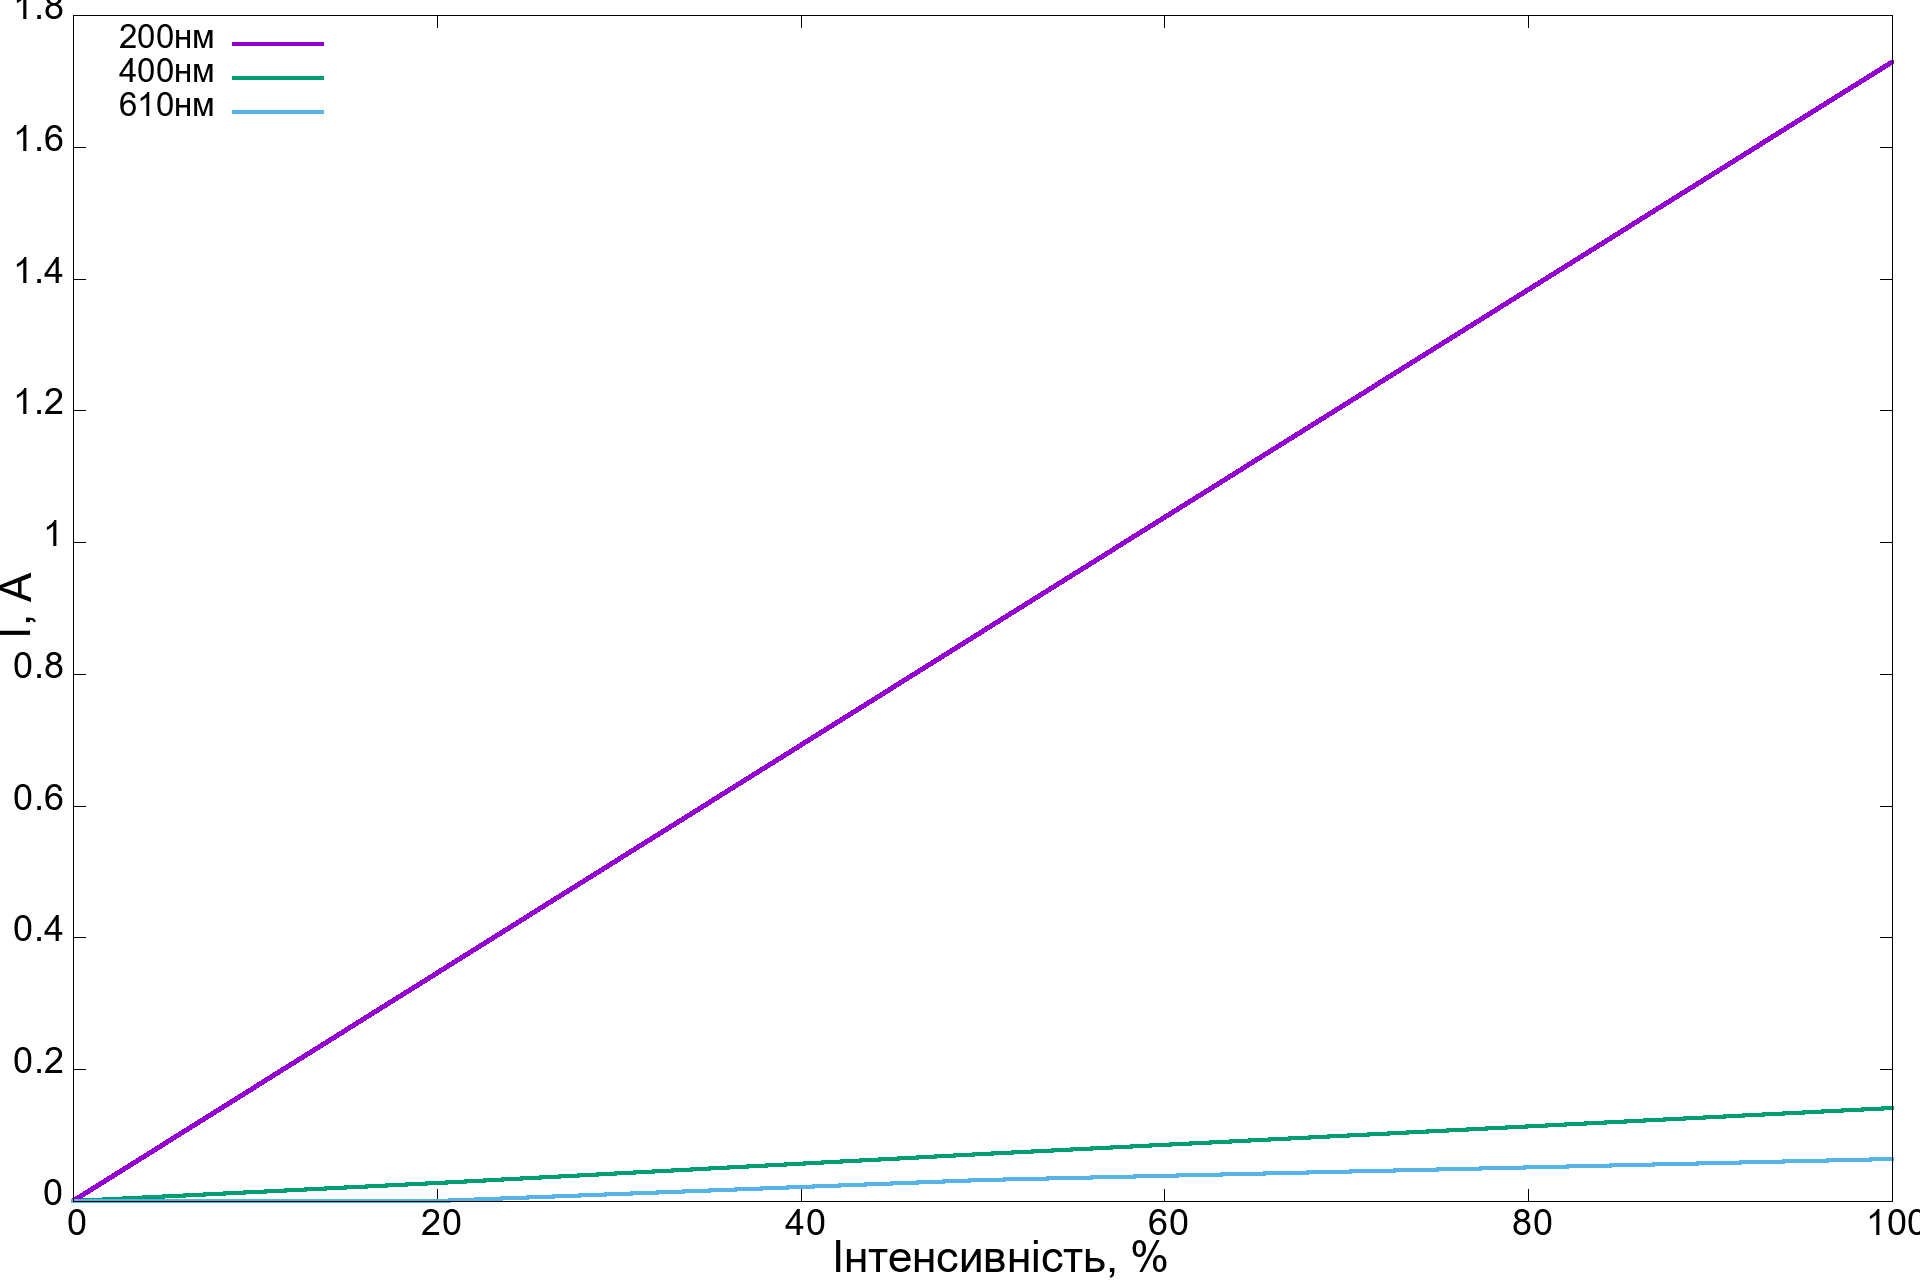
\includegraphics[width=0.9\linewidth]{2Na.png}}
\caption{Ciмейство кривих залежностi iнтенсивнлсті свiтла для довжин хвиль 200 нм, 400 нм, 440 нм для мiшенi з натрiя.}
\label{ris7}
\end{figure}

\newpage
\begin{center}\fbox{3}\end{center}
\begin{figure}[h]
\center{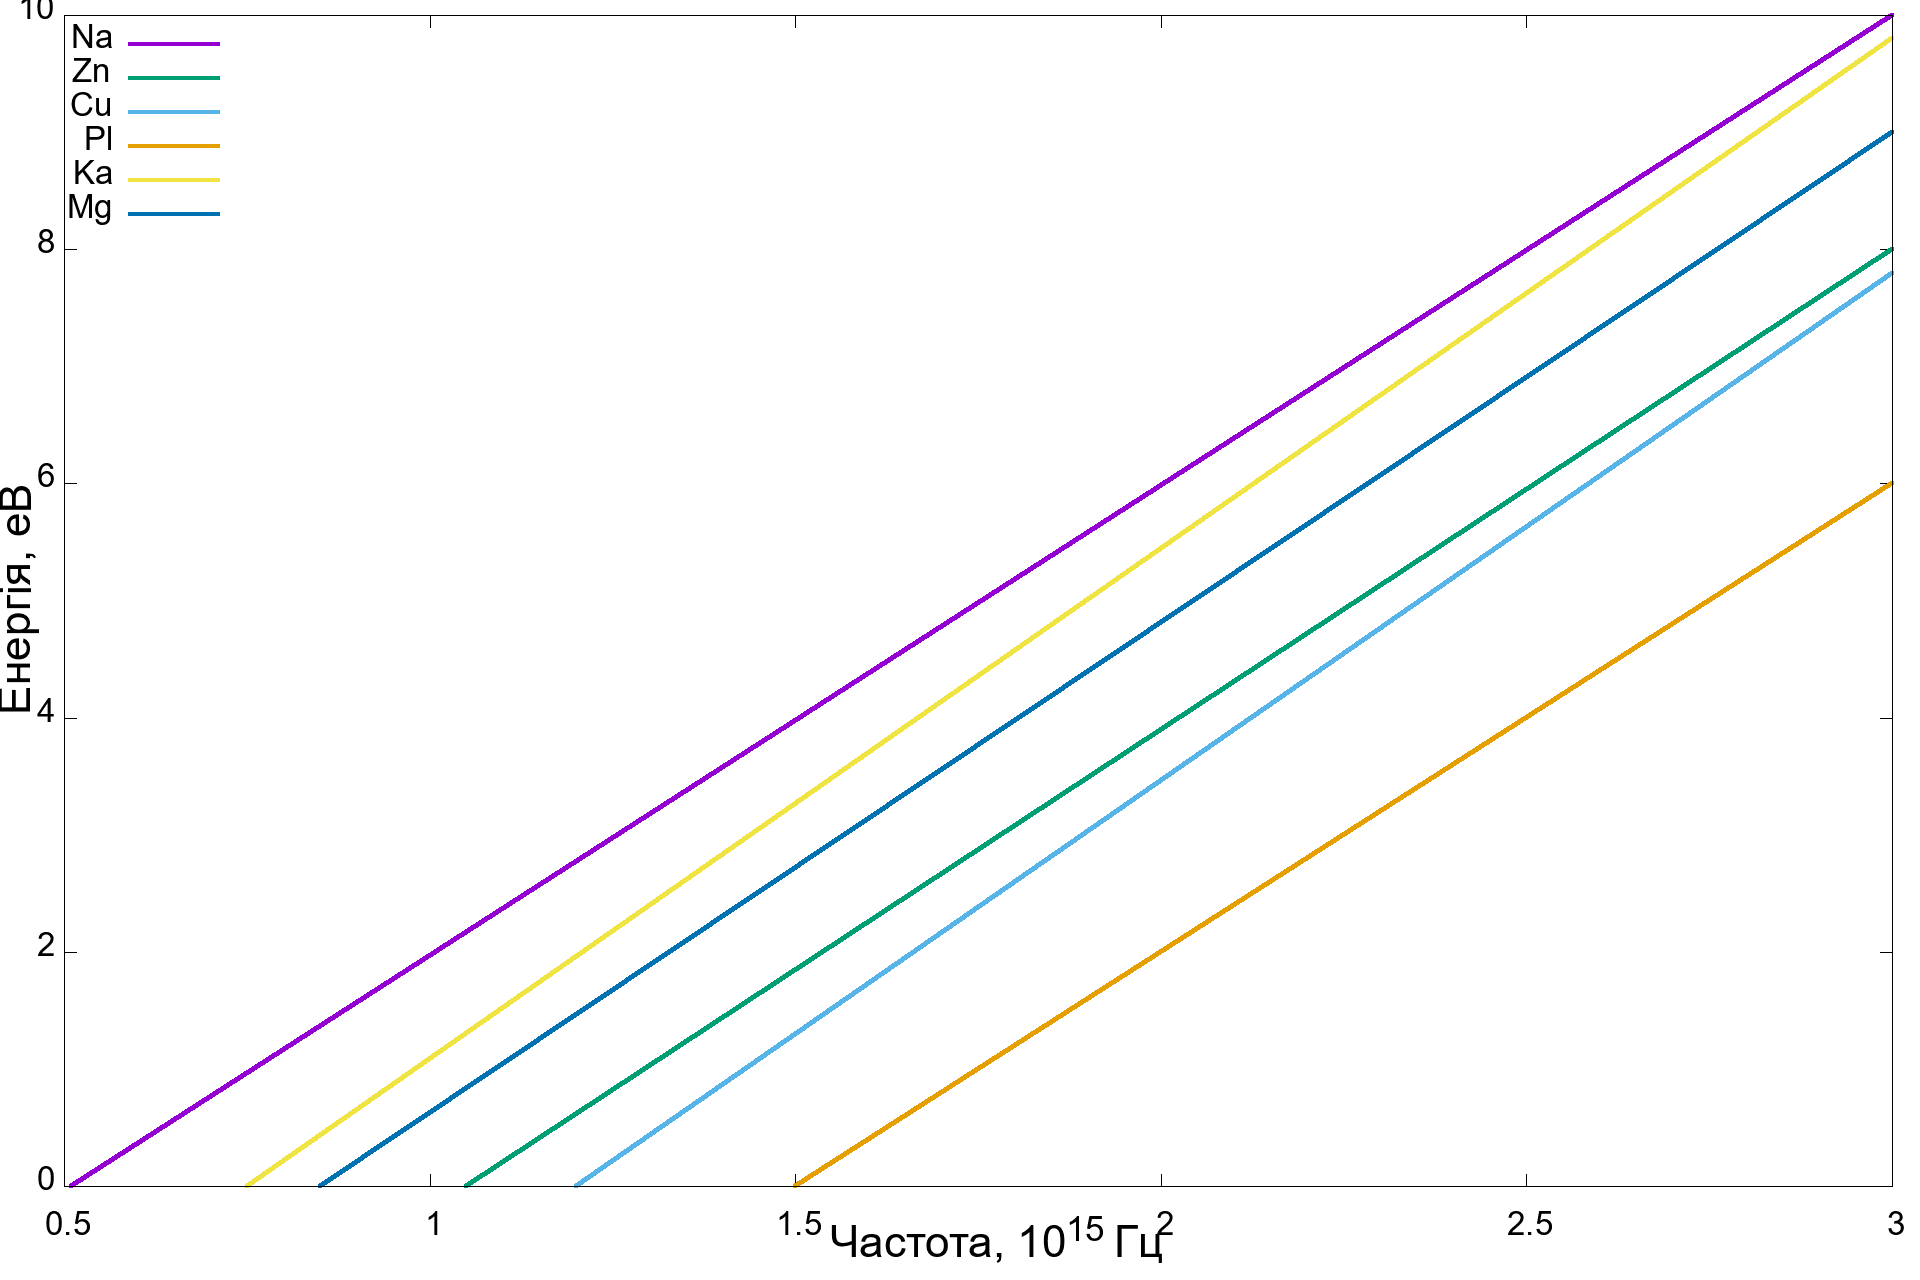
\includegraphics[width=0.9\linewidth]{3part.png}}
\caption{Ciмейство кривих залежностi Енергiя(частота) при iнтенсивностi 50\% на всьому iнтервалi частот для матерiалiв мiшенi: натрiй, цинк, мiдь, платина, кальцiй, магнiй.}
\label{ris8}
\end{figure}

\clearpage
\newpage
Висновок:\\
В ході лабораторної роботи ми дослідили вольт-амперні характеристики 
фотоелементів для видимого спектру світла.  
При порівнянні ВАХ металів
фотомішені, можна помітити, що найбільше значення фотоструму
характерне для натрію, оскільки натрій має найменшу роботу виходу, а найменше значення має мідь. 
Варто відмітити, що ВАХ за інтенсивності 50\% має менші 
значення, аніж при 100\% приблизно у два рази, це напевно через те, 
що при збільшенні величини світлового потоку емісія електронів буде збільшуватися, що в свою чергу буде впливати на саму величину струму насичення. 
Також помітно, що на короткій довжині хвилі интенсивність спостерігається набагато краще, а ніж на великій і при збільшенні самої інтенсивності також це видно. 
Кожен матеріал має своє граничне значення частоти та довжина хвилі світла, від яких залежить відбуватиметься фотоефект чи ні. 
За допомогою останнього сімейства можна зробити висновок, що при збільшенні частоти світла, енергія яку набувають електрони буде поступово збільшуватись. Також проаналізувавши останний рисунок можна визначити роботу виходу яка безпосередньо впливає на величину самого фотоструму. 
Виходячи з того, що  чим більше робота виходу, тим менше енергія електрона тому виходить, що  найбільше значення роботи виходу має платина, а потім вже йде мідь, цинк, магній, кальцій та натрій.
\end{document}
